\documentclass[]{article}

\usepackage{amsmath}  % AMS math package
\usepackage{amssymb}  % AMS symbol package
\usepackage{bm}       % bold math
\usepackage{graphicx} % Include figure files
\usepackage{dcolumn}  % Align table columns on decimal point
%\usepackage{multirow} % Multirow/column tables

\begin{document}
 

\title{PHY 905 Project 1: Monte Carlo simulation of the 2D ferromagnetic Ising model}

\author{Steve Hughey}

\date{\today}

\maketitle

\begin{abstract}
A simple Fortran implementation of the Metropolis algorithm for Monte Carlo simulation of the Ising model of ferromagnetism is described. Results are presented for energy and magnetization over a range of temperature.
\end{abstract}

\section{\label{sec:intro}Introduction}

\subsection{\label{sec:ising}Ising model}

The energy of the lattice is a sum over all nearest neighbor spin products, multiplied by an interaction strength $J$:
\begin{align}
H =& -J \sum_{<i,j>} s_i s_j
\end{align}

\section{\label{sec:imp}Implementation Details}

The change in energy due to negating the spin of a single point $i$ in the lattice is computed as the sum of $i$'s nearest neighbor spins multiplied by the new spin $s_i$ and the interaction strength $J$:

\begin{align}
\Delta E_i =& J s_i \sum_{<j>} s_j
\end{align}

\subsection{\label{sec:alg}Algorithm}

\section{\label{sec:res}Results}

The Fortran code implementing the 2D Ising model

\begin{figure}[ht!]
 \centering
 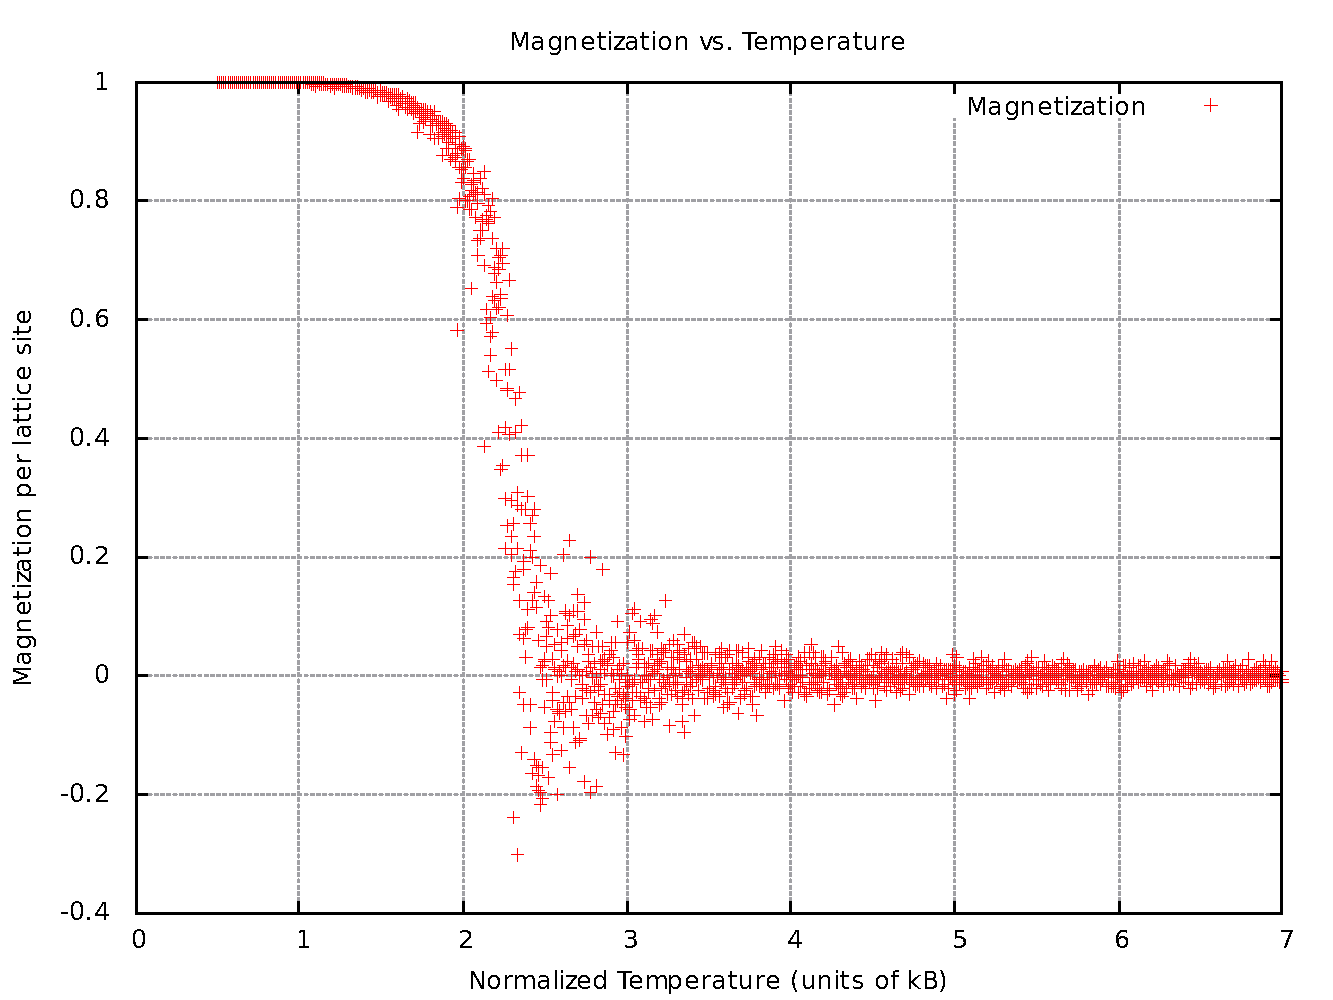
\includegraphics[width=\linewidth]{figures/mag_vs_temp.pdf}
 \label{fig:mag_vs_temp}
 \caption{Magnetization per lattice site. Values computed by averaging final 50000 Monte Carlo iterations per temperature value.}
\end{figure}

\begin{figure}[ht!]
 \centering
 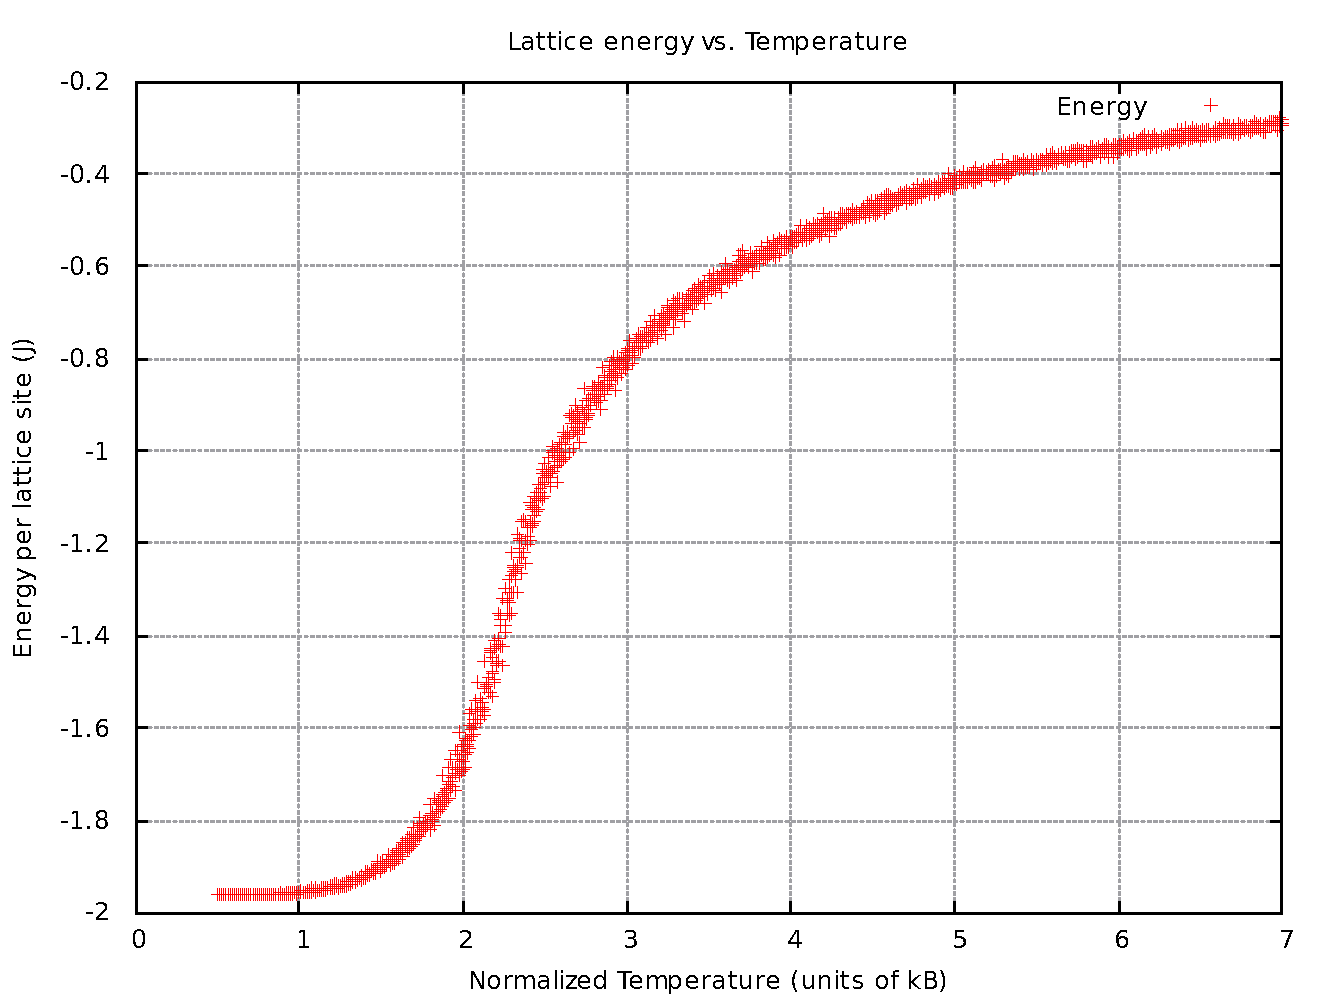
\includegraphics[width=\linewidth]{figures/energy_vs_temp.pdf}
 \label{fig:mag_vs_temp}
 \caption{Lattice energy per lattice site. Values computed by averaging final 50000 Monte Carlo iterations per temperature value.}
\end{figure}

\end{document}